\Chapter{Interprétabilité d'un modèle de classification par Attention Concentrée}\label{sec:Theme2}

Bien que partie intégrante du diagnostic des maladies rétiniennes \cite{boucherEvidencebasedCanadianGuidelines2020d}, l'utilisation de règles heuristiques ne s'appuyant que sur les lésions segmentées ne permet pas, en général, d'obtenir une classification automatisée robuste de la maladie, Ce constat est, dans une certaine mesure, confirmée par les résultats de notre précédent chapitre. Plusieurs éléments peuvent l'expliquer:
\begin{itemize}
	\item Les algorithmes de segmentation ne sont pas assez fiables; malgré leurs bonnes performances mesurées en comparaison avec une annotation manuelle produite par un expert.
	\item Les règles heuristiques définissant les étapes des maladies en fonction des lésions sont trop imprécises pour être strictement reproduites algorithmiquement.
	\item La définition de la maladie (ou de son grade dans le cas de la rétinopathie diabétique) varie selon le système de santé considéré. Par conséquence, les mêmes règles ne correspondent pas forcément au même stade pathologique.
	\item Lors du diagnostic, il existe une part d'interprétation subjective de l'image par le médecin qui use de son expérience et de son expertise. 
\end{itemize}
Cette dernière hypothèse peut s'interpréter sous le prisme du formalisme Bayésien: l'ensemble des diagnostics possibles suit une certaine distribution de probabilités, la décision du clinicien consiste à choisir celui qui minimise son incertitude étant données ses connaissances a priori et de toute autre information dont il dispose (incluant les lésions qu'il identifie dans l'image). 
Par opposition, le suivi strict d'en ensemble de règles heuristiques s'appuyant uniquement sur les lésions serait équivalent à une classification par arbre décisionnel. En simplifiant grandement, la première appartient au monde de l'apprentissage probabiliste, là où la seconde est du ressort de la logique symbolique (c'est à dire régit par des règles formelles non-ambiguës). \\
Comme cela a été présenté dans la revue de littérature (Chapitre \ref{sec:RevLitt} et en particulier dans la section \ref{sec:ReseauxNeurones}), l'essentiel des approches récentes sont statistiques et font usage de quantité massive de données. Ces données permettent aux réseaux de neurones d'extraire d'eux-même les marqueurs pathologiques via une représentation interne de l'image la plus souvent implicite. L'efficacité de ces approches est attestée dans de très nombreux cas, y compris pour des campagnes de dépistage de masse des principales maladies rétiniennes systémiques. En particulier, les travaux de Bhaskaranand et al.\cite{bhaskaranandValueAutomatedDiabetic2019a}, effectués sur plus de 100 000 visites de patients (soit 850 908 images) aboutissent à un système (désormais commercialisé) atteignant un couple sensibilité/spécificité de 91.3\% / 91.1\% pour la détection de la rétinopathie diabétique. De telles performances (ainsi que le volume de données utilisé dans l'étude, non accessible publiquement) rendent extrêmement ardue la quête d'un système plus performant. Cependant, plusieurs travaux pointent les limitations d'un tel modèle. Dans son éditorial pour la revue \textit{Nature}, Styles \cite{stylesIntroducingAutomatedDiabetic2019a} prend l'exemple du système de télédépistage Écossais qui s'appuie depuis 2012 sur un système automatisé pour effectuer un premier filtre des images saines. Si la complémentarité et la collaboration entre le système informatique et l'expert humain sont désormais bien acquises, la performance de la machine ne peut se réduire à un couple sensibilité/spécificité. En effet, dans certains cas, il existera une ambivalence, voire une opposition, entre l'expert humain et la machine. Il convient par conséquent d'anticiper ces cas. Or, il est difficile de trancher en cas de désaccord si les mécanismes de prise de décision du modèle sont inconnus (ce qui est généralement le cas avec des réseaux de neurones pouvant contenir plusieurs millions de paramètres). L'un des axes de recherches qui permet de résoudre ce problème vise à rendre interprétable les modèles employés, notamment a posteriori de leur entraînement. Un modèle cliniquement interprétable fournit à la fois un diagnostic précis et est également capable de souligner les structures locales de l'image qui l'ont guidé vers celui-ci. \\
Ayant ce contexte à l'esprit, l'objectif de notre travail de recherche est d'évaluer les performances d'un modèle récent de réseau de neurones reposant sur le principe de l'auto-attention appelé \textit{Vision Transformer}. Des performances élevées ont été obtenues dans plusieurs applications généralistes de reconnaissance d'images, mais parmi celles-ci, le domaine médical est encore peu exploré. Or, ces réseaux auto-attentifs permettent structurellement l'émergence d'une forme d'interprétabilité pouvant identifier les segments locaux de l'image qui ont conduit à la décision du modèle, contribuant ainsi à rendre le modèle interprétable par le médecin. Un aperçu de cette propriété était déjà promue dans l'article original des \ac{VIT}\cite{dosovitskiyImageWorth16x162020} et elle a par la suite été brièvement étudiée par Matsoukas et al. \cite{matsoukasItTimeReplace2021}, qui s'interrogent sur l'opportunité de remplacer les \ac{CNN}s par cette nouvelle architecture dans le domaine de l'imagerie médicale. Nous reprenons donc à notre compte l'hypothèse stipulant que la force (efficacité et acceptabilité) des réseaux auto-attentifs découlent structurellement de cette inhérente interprétabilité. \\
Dans ce chapitre, cette piste est explorée au travers de plusieurs scénarios mettant en jeu différentes types de données ophtalmologiques. L'interprétabilité du modèle ainsi conçu est évaluée sous le prisme de l'acceptabilité clinique par un panel de rétinologues expérimentés.
Pour tirer des conclusions générales, les expériences sont menées sur des données \ac{OCT} et de fond d'\oe il, car ces modalités présentent chacune des difficultés spécifiques. 
Par ailleurs, pour approfondir la compréhension du fonctionnement interne du réseau auto-attentif, nous proposons une étude du mécanisme d'extraction des patchs d'images et démontrons la possibilité d'améliorer la performance du modèle par ré-échantillonnage de ces patchs. Cette idée, particulièrement simple à mettre en place (elle ne nécessite pas d'entraînement et peut s'appliquer à n'importe quel modèle existant) a inspiré une technique originale appelée \og Attention Concentrée \fg (\textit{Focused Attention}) visant à produire des cartes d'interprétabilité en s'appuyant sur un schéma d'échantillonage conditionnel itératif permettant de filtrer progressivement les régions de l'image les plus pertinentes à sa classification. Pour valider à la fois notre hypothèse d'interprétabilité et d'efficience des modèles type \ac{VIT} par rapport à des \ac{CNN}s, nous évaluons les performances des modèles sur la classification de bases d'images de \fundus{} et \ac{OCT}, ainsi que sur la détection non-supervisée de lésions. Nous avons par ailleurs mis en place une étude randomisée auprès d'un panel de quatre ophtalmologistes expérimentés afin de leur évaluer différentes méthodes d'attributions générant des cartes d'interprétabilité (dont l'Attention Concentrée).
\\ 
Ainsi, pour résumer sommairement, les trois principales contributions présentées dans ce chapitre sont les suivantes:
\begin{enumerate}
	\item Évaluer quantitativement les performances de l'architecture \ac{VIT} et d'autres variantes et introduire un mécanisme de re-paramétrisation afin d'améliorer la précision du modèle en phase d'inférence. Cette étude met en jeu plusieurs modèles, bases de données et modalités pour tirer des conclusions couvrant un large panel de configurations.
	\item Proposer une nouvelle approche de la génération de carte d'interprétabilité appelée Attention Concentrée, reposant sur un échantillonnage conditionnel itératif des régions de l'image, donnant lieu à des cartes en hautes résolutions.
	\item Quantitativement et qualitativement valider l'interprétabilité intrinsèque des \ac{VIT} par rapport aux \ac{CNN}s en proposant un comparatif entre plusieurs méthodes.
\end{enumerate}

Ce chapitre est organisé de la sorte: la méthodologie employée est décrite dans la prochaine section \ref{sec:methodoFocusedAttention}, l'accent étant porté sur la notion de pas adaptatif et d'Attention Concentrée. Le protocole expérimental et les résultats sont détaillés dans la section qui suit \ref{sec:resultsFocusedAttention}. Nous en discutons la portée ainsi que les limitations de la méthode en section \ref{sec:discussionFocusedAttention}.
\section{Méthodologie}
\label{sec:methodoFocusedAttention}

Ce travail repose sur l'architecture originale du \ac{VIT}, dont le principe est décrit dans la sous-section qui suit; nos contributions -qui se greffent sur ce modèle- sont ensuite détaillées dans les deux sous-sections suivantes. Cette partie se conclue sur la description des stratégies d'entraînement, les jeux de données et les modules utilisés expérimentalement.
\subsection{Le modèle du \acl{VIT}}

Le \ac{VIT} consiste en une succession de couches d'encodages construites selon la même structure. Chaque couche $\mathbf{E}^n, n \in \{1,..., N\}$ ($N$ étant le nombre de couches) reçoit en entrée une séquence $S^n \in \mathbb{R}^{l\times d}$ composée de $l$ éléments (appelés \textit{jetons}) $s_i^n \in \mathbb{R}^d$ où $d$ représente la dimension de chaque jetons. À la différence des architectures de \ac{CNN}s typiques, où des opérations d'échantillonnage (\textit{pooling}) restreignent progressivement la résolution spatiale de l'entrée, pour le \ac{VIT}, la taille $l$ de la séquence reste inchangée de couche en couche. Pour la première couche, la séquence est obtenue par une projection linéaire de morceaux d'images (\textit{patches}) vers un vecteur de dimension $d$. Afin de maintenir l'information de positionnement spatial dans l'image de chaque jeton, on leur additionne un encodage positionnel. Enfin, la séquence ainsi constituée se voit greffer un jeton supplémentaire, dit de \textit{classification}.
Tel que représenté sur la figure \ref{fig:ViTEncoderBlock}, la propagation au sein d'une couche d'encodage se fait en plusieurs étapes:
\begin{enumerate}
	\item Chaque séquence est d'abord normalisée, utilisant la technique de Ba et al. \cite{baLayerNormalization2016} dite de \og Normalisation par Couche \fg (\textit{\ac{LN}}).
	\item Elle est recomposée via une opération auto-attentive. Celle-ci est réalisée parallèlement $K$ fois, d'où l'appellation originale de \textit{\ac{MHA}}.
	\item La sortie du MHA est fournie à un réseau de neurones à deux couches, utilisant la fonction d'activation de type \textit{\ac{GELU}}.
\end{enumerate}
Par ailleurs, le \ac{VIT} utilise deux connexions résiduelles au sein d'une couche. L'ensemble de ces étapes se résume donc par le jeu d'équations suivant:
\begin{align}
	S^{n}_{a} &= \text{MHA}(\text{LN}(S^{n-1})) \\ 
	S^{n}_{b} &= S^{n}_{a} + S^{n-1} \\
	S^{n} &= \text{MLP}(\text{LN}(S^{n}_b)) + S^{n}_{b}
\end{align}
Il reste à décrire le principe de fonctionnement de la couche \ac{MHA}. Chaque jeton $s_i^n$ est projeté vers trois composantes distinctes appelées Clé, Requête et Valeur (respectivement \textit{Key, Query, Value} dans leur nom original) et notées $k_i^n$, $q_i^n$, $v_i^n$. Ces trois vecteurs s'obtiennent par la projection linéaire de chaque jeton d'entrée, ce qui donne, sous forme d'équation matricielle:
\begin{align}
	K^n &= I^n \cdot W^n_k \\
	Q^n &= I^n \cdot W^n_q \\
	V^n &= I^n \cdot W^n_v \\
\end{align}
où $I^n = \text{LN}(S^{n-1})$ représente la séquence de jetons normalisée. Une tête d'attention $A^n$ est obtenue par le produit de la matrice de Clé et de Requête:
\begin{equation}
	A^n = \frac{Q^n \cdot K^{nT}}{\sqrt{d}}
\end{equation}
On en extirpe une matrice de scores d'importance par jetons normalisée via la fonction $\text{softmax}$ appliquée ligne-à-ligne, permettant ainsi de pondérer la dépendance entre chaque paire de jetons dans la séquence.
Le \ac{MHA} s'obtient alors comme:
\begin{equation}
	S^{n}_{a} = \text{softmax}(A^n)V^n
\end{equation}
\begin{figure}[tbh!]
	\centering
	\includegraphics[width=.6\textwidth]{focused_attention/architecture/architecture}
	\caption{Représentation d'une architecture \ac{VIT} utilisée sur la classification d'une image OCT. Le modèle se compose d'une succession de $N$ couches d'encodage. Le jeton de classification de la dernière couche est fourni en entrée d'une régression linéaire dont la sortie représente la décision du modèle.}
	\label{fig:ViTEncoderBlock}
\end{figure}

\subsection{Affinage de l'attention par ajustement du pas}
\label{sec:adaptativeStride}
Nous proposons une méthode simple et qui peut s'étendre à n'importe quel type de modèle à base de jetons dérivé du ViT. Dans sa publication originale \cite{dosovitskiyImageWorth16x162020}, le \ac{VIT} décompose une image d'entrée en patchs adjacents non superposés, projetés sur des vecteurs unidimensionnels et fournis au modèle sous la forme d'une séquence de jetons individuels.
Cette opération est réalisée via une simple convolution dont la taille du noyau et le pas déterminent la taille de chaque patch et le chevauchement entre eux. Or, étant donné que la matrice d'attention est calculée à l'échelle des jetons, nous émettons l'hypothèse qu'augmenter leur nombre peut améliorer le modèle en fournissant des patchs supplémentaires centrés sur davantage d'éléments structurels de l'image. Cette augmentation se fait tout simplement en diminuant le pas de la convolution projective. Ce faisant, on obtient une forme d'agrandissement de la résolution de la séquence, d'où le choix de parler d'échelle d'échantillonnage par la suite. Comme chaque élément de la séquence est accompagné de son encodage positionnel, à chaque échelle, de nouveaux encodages doivent être calculés pour les jetons sur-échantillonnés. Si ceux-ci sont définis de manière formelle et analytique (sur la base de la position du patch dans l'image), leur calcul pour les nouveaux patchs est simple. Pour nos expériences, nous avons fait le choix d'un encodage appris au cours de l'entraînement.
Dans ce cas, l'obtention d'un nouveau vecteur d'encodage lors du sur-échantillonnage de la séquence se fait simplement par interpolation des encodages existants entre ceux des jetons adjacents. Cette interpolation ne nécessite pas de ré-apprentissage, et de manière générale, l'ensemble de ce processus est conçu pour ne s'appliquer qu'à l'inférence sur un modèle pré-existant, sans modification intrinsèque de ses poids. Néanmoins, la relation entre le nombre de jetons et la taille du matrice d'attention est quadratique. C'est également le cas pour la relation entre le pas de la convolution projective et le nombre de jetons. En d'autres termes, une division par $k$ du pas de convolution entraîne une augmentation par $k^4$ de la taille de la matrice d'attention à calculer.
Ce effet a pour corollaire le risque d'une rapide saturation de la mémoire graphique nécessaire pour effectuer les calculs d'attention.
Dans ces conditions, l'applicabilité de l'approche reste limitée au matériel haut de gamme, même pour une seule image et simplement à l'inférence (c'est-à-dire lorsque la rétro-propagation des gradients n'est pas nécessaire). Ce fait justifie la poursuite de la recherche vers des techniques d'échantillonnage plus efficaces.

\subsection{L'Attention Concentrée: un ré-échantillonnage itératif conditionnel}

L'inconvénient du ré-échantillonnage naïf du nombre de jetons est liée à des limitations matérielles sur la mémoire graphique disponible. La quantité de mémoire nécessaire augmente exponentiellement avec le facteur de division du pas de la convolution projective. Cette contrainte la rend en l'état incompatible avec toute forme de technique qui requiert la rétro-propagation des gradients, ce qui est notamment le cas pour l'essentiel des approches d'interprétabilité pour la génération de cartes d'attributions. On peut cependant arguer que tous les patchs ne sont pas de la même importance pour la classification d'une image et a fortiori pour le diagnostic. Intuitivement, pour ce dernier cas de figure, les plus importants seront ceux centrés sur des lésions ou des marqueurs anormaux de l'image. La méthode proposée exploite cette hypothèse et consiste à générer une carte d'attribution et une prédiction en n'utilisant qu'un sous-ensemble des jetons pour chaque échelle (au sens donné dans la section précédente). Choisir ce sous-ensemble revient à attribuer un score d'importance par jetons et à filtrer les moins importants. Un tel score n'est naturellement pas trivial, mais c'est précisément le rôle que remplissent les algorithmes de générations de cartes d'attributions tels que l'\textit{Attention Rollout} ou \ac{LRP}. De tels algorithmes permette d'indiquer les jetons de la séquence qui ont le plus contribué à la prédiction du modèle. Par extension, ils peuvent donc servir à définir des régions d'intérêts dans l'image, permettant un ré-échantillonnage des jetons dans la zone considérée. \\
Pour ce faire, on définit un processus itératif au travers d'une échelle de pas de convolution décroissants $s_i, i \in \{1,...,M\}$. Par simplification, on ne considère que des pas sous forme de puissance de deux, $s_i = \frac{s_0}{2^i}$, $s_0$ étant le pas du modèle originel. Notre procédure s'initie généralement avec $s_0=32$ ou $s_0 = 16$ et fait décroître  $s_i$ jusqu'à $s_M=1$. En pratique, n'importe quel entier entre $s_0$ et $1$ convient. 
À $s_0$, le réseau est utilisé de manière classique, c'est-à-dire tel qu'il a été entraîné. Lors de cette étape d'initialisation, une carte d'attribution est générée via une méthode arbitrairement choisie, produisant un score pour chaque élément de la séquence de jetons. Celle-ci est ensuite sur-échantillonnée (par la méthode du pas décroissant décrit dans la section précédente). À cette nouvelle échelle, seul un sous-ensemble de ces nouveaux jetons sont fournis au réseau. La sélection de ceux-ci se fait par un échantillonnage aléatoire conditionnel basé sur le score d'attribution obtenu à l'échelle précédente. Le sous-ensemble est maintenu de taille constante $P$, de telle manière à contenir le calcul de la matrice d'attention à une taille $P+1 \times P+1$ ($P$ jetons sélectionnés et un jeton de classification). Expérimentalement, nous avons aussi observé qu'ajouter les patchs adjacents (dans l'image) à ceux sélectionnés par échantillonnage conditionnel améliorent les résultats. Il est vraisemblable que ceux-ci permettent d'amener un contexte local autours des patchs choisis. \\
La quantité $P$ de jetons conservés devant rester modérée du fait des contraintes matérielles, nous répétons l'opération d'échantillonnage conditionnel $K_i$ fois par échelle $s_i$, ce qui se traduit par $K_i$ inférence par échelle. Cela a pour effet d'augmenter le nombre effectif de jetons considérés de $P \times K_i$ par échelle et par image tout en maintenant les exigences en mémoire constantes. Étant donné que le nombre de jetons se densifie au fur et à mesure des échelles, on accroît le nombre d'étapes de ré-échantillonnage par échelle de manière progressive suivant l'équation $K_i = \lfloor 1.5^i \rfloor$ (où $\lfloor x \rfloor$ est l'arrondi à la plus petite valeur entière la plus proche de $x$).
Les $K_i$ cartes d'attributions produites par échelle sont fusionnées en une seule carte, elle-même agrégée aux précédentes cartes générées aux échelles inférieures. Nous avons expérimenté avec deux fonctions d'aggrégation: la moyenne et le maximum élément-par-élément; les résultats les plus probants étant obtenus avec la première. Pour chaque échelle $s_i$, la carte d'attribution est deux fois plus petite que celle produite à l´échelle suivante: si on souhaite s'en servir comme carte conditionnel d'échantillonnage, il est donc nécessaire de la redimensionner, ce que nous faisons par interpolation bilinéaire. Le processus complet se résume donc à $\sum_{i=1}^{M} K_i$ inférences et à l'aggrégation d'autant de cartes d'attributions. \\
Nous nommons cet algorithme \textit{l'Attention Concentrée}: en effet, il vise à condenser le calcul de l'attention sur les zones de la séquence d'entrée les plus pertinentes. La figure \ref{fig:focusedattentionmechanism} illustre le fonctionnement simplifié du processus. Le pseudo-code détaillé correspondant est fourni (Algorithme \ref{algo:pseudoCodeFocusedAttention}). Quelques exemples du processus d'aggrégation de la carte d'attribution finale sont données sur la figure \ref{fig:FocusedAttentionExamples}
\begin{figure}[htb]
	\centering
	\includegraphics[width=.8\textwidth]{gnuplot/focused_attention/focusedAttention/focusedAttentionMechanism}
	\caption{Mécanisme illustré de l'Attention Concentrée}
	\label{fig:focusedattentionmechanism}
\end{figure}

\begin{figure}[!h]
	\begin{subfigure}{\textwidth}
		\includegraphics[width=\textwidth]{gnuplot/focused_attention/focusedAttention/Example_0}
	\end{subfigure}
	\begin{subfigure}{\textwidth}
	\includegraphics[width=\textwidth]{gnuplot/focused_attention/focusedAttention/Example_2}
	\end{subfigure}
\begin{subfigure}{\textwidth}
	\includegraphics[width=\textwidth]{gnuplot/focused_attention/focusedAttention/Example_3}
\end{subfigure}
\begin{subfigure}{\textwidth}
	\includegraphics[width=\textwidth]{gnuplot/focused_attention/focusedAttention/Example_4}
\end{subfigure}
\caption{Exemples de la reconstruction de la carte d'attribution haute résolution par Attention Concentrée. Chaque colone représente un pas différent de l'opérateur de projection convolutif. L'avant dernière et la dernière colonnes représentent respectivement l'attribution finale et la vérité terrain des lésions contenues dans l'image.}
\label{fig:FocusedAttentionExamples}
\end{figure}

\begin{algorithm}[!h]
	\caption{Pseudo-code pour l'Attention Concentrée}
	\label{algo:pseudoCodeFocusedAttention}
	\begin{algorithmic}[1]
		
		\State $s \gets 32$ \Comment{Pas initial}
		\State $P \gets 256$ \Comment{Quantité de jetons échantillonnés}
		\State $attr  \gets obtenirCarteAttribution(model)$	\Comment{Obtention de l'attribution originale (LRP, Rollout...)}
		\State $i \gets 0$
		\While{$s>=1$}
		\State $i \gets i+1$
		
		\State	$s \gets \frac{s}{2}$
		\State $model.stride \gets s$
		\State $reechantillonnageEncodagePositionnel(model, s)$
		\State $attr \gets interpolate(attr)$ \Comment{Interpolation de la carte d'attribution}
		\State $cdf = cumsum(attr)$ \Comment{Obtention de fonction de répartition de la distribution d'échantillonnage des jetons}
		\State $K = \lfloor 1.5^i \rfloor$
		\For{$k \gets 0$ à $K$}
		\State $u \gets uniform(P)$ \Comment{Échantillonnage d'un vecteur de taille P suivant une loi de distribution uniforme}
		\State $indices \gets searchsorted(cdf, u)$ \Comment{Utilisation de la fonction de répartition conditionnelle pour choisir les jetons conditionnellement à l'attribution}
		\State $voisins \gets chercheVoisins(indices)$
		\State $indices.append(voisins )$
		\State $model.keptIndices \gets indices$ \Comment{Le modèle ne conserve que ces jetons}
		\State $newAttr \gets obtenirCarteAttribution(model)$
		\State $attr[indices] \gets aggrege(attr[indices], newAttr)$
		
		\EndFor
		\EndWhile
	\end{algorithmic}
\end{algorithm}

\subsection{Entraînement des modèles}
Pour vérifier l'efficacité et la capacité de généralisation du \ac{VIT} avec pas ajusté et Attention Concentrée, nous avons entraîné plusieurs modèles sur deux modalités d'imagerie distinctes. La grande majorité des éléments d'entraînements est conservée à l'identique entre les deux modalités; néanmoins, certains hyperparamètres doivent être ajustés à chacune. Tous les modèles sont soient entièrement ré-implémentés, soit dérivés des modèles fournis par la librairie de référence TIMM de R. Wightman \cite{wightmanPyTorchImageModelsWightman}. 

\paragraph{OCT} Les modèles sont entraînés pour la minimiser la fonction d'entropie-croisée avec lissage des labels (\textit{label smoothing}) proposée par Szegedy et al.\cite{szegedyRethinkingInceptionArchitecture2016}. Une pondération par classe est ajoutée pour contrebalancer le déséquilibre de classe existant dans nos données. L'optimisation se fait par Descente de Gradients Stochastiques avec une inertie (\textit{Nesterov's momemtum}) de 0.9, un pas d'apprentissage de 0.0002 et une régularisation sur la norme $\text{L}_2$ des poids de 0.005 (\textit{weight decay}). On utilise un planificateur de pas d'apprentissage, pour diviser celui-ci par 2 dès que le modèle atteint un plateau de performance (la \acl{mIoU}) sur l'ensemble de validation. 

\paragraph{Fond d'\oeil} Le pas d'apprentissage est fixé à 0.001. On augmente également le nombre d'itérations d'apprentissage. Hormis cela, les hyperparamètres sont les mêmes que pour l'OCT. De l'augmentation de données à la volée est employée grâce à la librairie Albumentations de Buslaev et al. \cite{info11020125} et consiste en des rotations et des mises à l'échelle aléatoires ainsi que des ajustements colorimétriques (luminosité, contraste, teinte...).

\subsection{Bases de données}
\label{sec:databaseFocusedAttention}
\paragraph{OCT} La majorité des expériences est menée sur la base de données UCSD \ac{OCT} publiée par Kermany et al. \cite{kermanyIdentifyingMedicalDiagnoses2018} en 2018. Elle contient 108309 B-scans, rangés en quatre classes: Normal, présence de drusens, de Néo-vascularisation choroïdale ou d'\oe dème  diabétique maculaire. Parmi ce jeu, 1000 images ont été aléatoirement extraites pour être utilisées en tant qu'ensemble de validation. La base UCSD propose également un ensemble de test indépendant de 1000 images, parfaitement équilibré entre les quatre classes. Parallèlement, nous avons collecté 324 B-scans dont l'acquisition est faite à l'\ac{HMR} de Montréal. Ces images ont été annotées par un expert de de la rétine pour correspondre aux quatre même classes présentes dans UCSD et ont servi comme ensemble de test complémentaire. Pour quantifier les performances des segmentations par carte d'attribution, nous utilisons la base de données AROI, publiée par Melinščak et al.\cite{melinscakAnnotatedRetinalOptical2021} en 2021. Ce jeu contient 1136 B-scans, pris sur 24 patients atteints de dégénérescence maculaire liée à l'âge au stade néovasculaire. Pour chaque image, des cartes de segmentation sont fournies, indiquant la présence des poches de fluides rétiniens anormales (détachement de l'épithélium pigmentaire, liquide sous-rétinien et intrarétinien). Ces biomarqueurs sont en lien avec les quatre classes de la base de données UCSD. Par exemple, un détachement de l'épithélium peut être dû à une accumulation d'exsudats doux. \\
\paragraph{Fond d'\oeil} Trois bases de données distinctes ont été utilisées pour évaluer notre méthodologie sur les images de \fundus. La base de données EyePACS, introduite par Cuadros et Bresnick en 2009 \cite{cuadros_bresnick_2009} et popularisée par une compétition organisée sur la plateforme Kaggle, contient un ensemble d'entraînement et d'évaluation de 35 126 et 53 576 images respectivement. Deux configurations ont été expérimentées: 
\begin{itemize}
	\item Apprentissage en faible régime de données, n'utilisant que l'ensemble d'entraînement.
	\item La combinaison des deux ensembles (pour un total de 88 702 images).
\end{itemize}
Pour cette deuxième configuration, comme il est bien nécessaire d'évaluer le modèle sur un ensemble séparé, une autre base de données est mise en jeu. Il s'agit de la base Aptos, également rendue publique lors d'une compétition Kaggle en 2019 \cite{APTOS2019Blindness2019}. Elle contient 3 662 images que nous n'avons utilisées que pour l'évaluation des modèles. Aptos et EyePACS sont de structures similaires, toutes deux contenant des images associées chacune aux cinq grades de rétinopathie diabétique (aucune, légère, modérée, sévère et proliférative). Cependant, les deux bases se distinguent par l'origine des patients, par la qualité des images et par la distribution des classes. \\
En supplément, nous avons également utilisé la base de données \ac{IDRiD} \cite{porwalIDRiDDiabeticRetinopathy2020}, pour laquelle tous les détails sont données dans le chapitre \ref{sec:ChapitreSegmentation}. Pour toutes ces images, un même pré-traitement est appliqué, consistant à centrer l'image sur sa région d'intérêt en retirant au maximum les bordures noires (voir la section \ref{sec:resolution_standardisation} pour la méthodologie exacte). La résolution standardisée choisie est de $384 \times 384$.

\subsection{Architectures neuronales}
En termes de modèles de référence, nous avons utilisé trois différents \ac{CNN}s: le ResNet-152 \cite{heDeepResidualLearning2016a}, le Wide-ResNet-101 \cite{zagoruykoWideResidualNetworks2016} et l'Optic-Net 71 \cite{kamranOpticNetNovelConvolutional2019} de Kamran et al. spécialement conçus pour la classification des images OCT. Ce dernier modèle n'ayant pas convergé sur la classification des images de \fundus{}, nous l'avons remplacé sur ces dernières par un EfficientNet B7. Le choix de ce modèle est motivé par ses performances au sommet de l'état de l'art sur la base de données ImageNet. \\
Dès lors ces références choisies, nous avons configuré nos expériences sur plusieurs modèles de type auto-attentifs (\textit{Transformers}) en faisant varier leur architecture (ViT, DeiT, T2T-ViT) et leur nombre de paramètres. Dans les résultats fournis par la suite, ces modèles sont nommés suivant la nomenclature existante dans la librairie TIMM \cite{wightmanPyTorchImageModelsWightman} (d'où sont également issues les poids pré-entraînés). Le suffixe \og base\fg se réfère à un modèle utilisant espace latent de taille 768, une profondeur de 12 couches et 12 têtes d'attention par couche. Le suffixe \og large \fg indique respectivement des valeurs 1024, 24 et 16 pour ces mêmes dimensions. Par ailleurs, nous indiquons entre parenthèses la taille du pas initial de la convolution projective (plus le pas est grand, moins la séquence l'est). Enfin, pour le modèle T2T-ViT, l'espace latent est choisi de taille 512 et trois configurations sont expérimentées, correspondant à des profondeurs de 14, 19 et 24 couches.

\subsection{Hiérarchisation des méthodes d'interprétabilité par attribution}
Notre objectif premier n'est pas nécessairement de déterminer quel modèle est le plus performant mais de savoir lequel est perçu comme pertinent dans un contexte clinique. Bien entendu, la pertinence est jugée à l'aune de sa performance de classification, mais également de sa capacité à fournir une prédiction interprétable, c'est-à-dire de justifier son diagnostic d'une manière ou d'une autre. Pour cela, nous avons fait le choix d'étudier les capacités d'interprétabilité visuelle (voir la section \ref{sec:interprétabilitéModel} pour un état de l'art sur le sujet). Plusieurs médecins ont été mis à contribution pour évaluer leur appréciation de différentes cartes d'attributions, générées par plusieurs modèles et en utilisant diverses méthodes d'attribution existantes et l'Attention Concentrée que nous proposons. 
\\
Pour mener à bien ce sondage, nous avons développé une plateforme accessible depuis un navigateur, permettant d'inspecter les images et leur carte d'interprétabilité respective. Une capture d'écran de l'outils est montrée sur la figure \ref{fig:surveyinterface}. L'outils permet de naviguer dans la base de données d'images, hébergée sur un serveur privé de l'École Polytechnique. Pour chaque expert, une connexion sécurisée est assurée par un service externe (\textit{auth0}\footnote{\url{https://auth0.com/}}). L'ouverture d'une session sur la plateforme envoie une requête vers un serveur développé en Python avec le micro-framework Flask \footnote{\url{https://flask.palletsprojects.com/en/2.2.x/}}. Les images, leurs cartes d'attributions associées, les comptes des médecins et les annotations qu'ils réalisent sont stockés sur différentes tables SQL. 
\\ 
Pour une même image, les cartes d'attributions sont présentées selon un ordre aléatoire, sans préciser la nature de l'algorithme sous-jacent avant d'éviter de biaiser l'évaluateur humain. Il lui est possible de zoomer dans chaque image, d'agrandir l'interface et de contrôler l'opacité de la carte d'attribution superposée à l'image. Il associe à chaque carte un score compris entre 1 et 5.
\begin{figure}
	\centering
	\includegraphics[width=\linewidth]{focused_attention/survey/survey_interface}
	\caption{Capture d'écran de l'interface de la plateforme développée dans le cadre du sondage sur l'interprétabilité des réseaux neuronaux mené auprès d'experts médicaux.}
	\label{fig:surveyinterface}
\end{figure}

\section{Protocole expérimental}
\label{sec:resultsFocusedAttention}
Notre protocole est organisé comme suit: tous les modèles sont entraînés dans les mêmes conditions, afin de garantir une comparaison non biaisée et souligner ainsi leurs forces et faiblesses. Le même budget en terme d'itérations d'apprentissage est donc alloué à chaque modèle. Sur les deux modalités, les modèles sont testés sur plusieurs ensembles d'évaluation. En second lieu, nous évaluons l'impact du concept de pas adaptatif décrit dans la section \ref{sec:adaptativeStride}. Enfin, la dernière étape est consacrée à l'évaluation des cartes d'attributions générées par divers algorithmes. 
\subsection{Performance de classification}
\paragraph{OCT} Afin de comparer les performances des différents modèles, nous avons calculé la précision, la sensibilité, la spécificité et l'exactitude sur les différents ensemble d'évaluation. Pour l'ensemble UCSD, les résultats sont données dans le tableau \ref{tab:CNN vs ViT-OCT}. Ils permettent d'illustrer la capacité des \ac{VIT} à égaler les \ac{CNN}s dès lors que le réseau est suffisamment complexe et utilisant des petits patchs. Cela se paye en contrepartie par une augmentation drastique des ressources nécessaires pour faire fonctionner le modèle. Le modèle \ac{VIT} le plus performant de notre échantillon est le ViT\textsubscript{base}\textsuperscript{(16)}, obtenant une exactitude de 97.80\% (soit presque égale à celle Wide ResNet101 de 98\%). Cependant, ce modèle est significativement plus complexe que les autres en nombre d'opérations élémentaires requises pour une passe d'inférence. On note par ailleurs des performances en deçà de celles attendues pour les modèles de type T2T-ViT, mais également une complexité bien moindre. 

\begin{table*}[!h]
	\caption{Performances comparées entre les modèles de référence de types \ac{CNN}s et les modèles \ac{VIT} pour la classification des OCTs de la base UCSD. Le nombre de paramètres (en millions) et le nombre approximatif d'opérations élémentaires d'addition/multiplications (\textit{Multiply-Add Count} (MAC)) pour l'inférence sur une image sont donnés à titre indicatif sur la complexité des modèles.}\label{tab:CNN vs ViT-OCT}
	\centering
	\begin{tabularx}{\textwidth}{Xcccc||cc}
		\hline
		Modèles &  Exactitude & Spécificité &  Précision & Sensibilité & Params. (M) & MACs (G) \\ % PHD: petites modifs ici
		\hline
		\multicolumn{7}{c}{Modèles de référence} \\
		\hline
		Wide ResNet101  & \textbf{98.00} & \textbf{99.33} & \textbf{98.15} & \textbf{98.00} & 477 & 124.85\\
		Optic-Net71  & 96.80 & 98.93 & 97.06 & 96.80 & 48 & 12.45 \\
		ResNet152 & 96.40 & 98.80 & 96.61 & 96.40 & 223 & 58.15 \\
		\hline
		\multicolumn{7}{c}{Modèles auto-attentifs} \\
		\hline
		ViT\textsubscript{base}\textsuperscript{(32)}  &96.00 & 98.67 & 96.43 & 96.00 & 87 & 10.98 \\
		ViT\textsubscript{base}\textsuperscript{(16)} &94.80 & 98.27 & 95.55 & 94.80 & 86 & 47.31 \\
		
		ViT\textsubscript{large}\textsuperscript{(32)} &90.20 & 96.73 & 92.40 & 90.20 & 303 & 162.0 \\
		
		ViT\textsubscript{large}\textsuperscript{(16)} &97.80 & 99.27 & 97.93 & 97.80 & 303 & 162.0 \\
		DeiT\textsubscript{base}\textsuperscript{(16)} &95.80 & 98.60 & 96.28 & 95.80 & 86 & 47.40 \\
		T2T-ViT\textsubscript{14} &94.40 & 98.13 & 94.91 & 94.40 & 21.5 & 6.1 \\
		T2T-ViT\textsubscript{19} &93.20 & 97.73 & 94.40 & 93.20 & 39.2 & 9.8 \\
		T2T-ViT\textsubscript{24} &93.40 & 97.80 & 94.67 & 93.40 & 64.1 & 15.0 \\
		\hline
	\end{tabularx}
\end{table*}

En ce qui concerne la généralisation sur des données externes, les performances sur la base d'évaluation \ac{HMR} sont bien moindres pour tous les modèles (voir le tableau \ref{tab:performance-HMR data}). En moyenne, on observe une baisse de 7.51\% tous modèles confondus. Dans le détail, elle est de 7.77\% pour les CNNs, 7.97\% pour les VITs et de 6.63\% pour les T2T-ViTs. Bien que cela puisse indiquer une meilleure capacité de généralisation pour ces derniers, étant donnée la taille limitée de la base de test et du nombre de modèles considérés, aucune conclusion ferme ne peut être tirée. Enfin, notons la relativement haute performance obtenue par le Optic-Net71, dépassant tous les modèles, y compris le ViT\textsubscript{base}\textsuperscript{(16)} (deuxième de notre classement) de plus de 2\%.

\begin{table}[!h]
	\caption{Performances comparées sur la classification des OCT de la base \ac{HMR}.}
	\label{tab:performance-HMR data}
	\centering
	% \addtolength{\tabcolsep}{+0pt}
	
	\begin{tabularx}{\columnwidth}{Xcccc}
		\hline
		Modèles &  Exactitude & Spécificité &  Précision & Sensibilité\\
		\hline
		\multicolumn{5}{c}{Modèles de référence} \\
		\hline
		Wide ResNet101  &   89.51 & 96.62 & 91.39 & 88.49 \\
		Optic-Net71  &   \textbf{92.59} & \textbf{97.62} & \textbf{93.22} & \textbf{91.96}\\
		ResNet152 &   85.80 & 95.40 & 89.19 & 84.42 \\
		\hline
		\multicolumn{5}{c}{Modèles auto-attentifs} \\
		\hline
		ViT\textsubscript{base}\textsuperscript{(32)}  & 87.65 & 95.95 & 90.07 & 86.21\\
		ViT\textsubscript{base}\textsuperscript{(16)} &  88.27 & 96.15 & 89.44 & 87.31\\
		ViT\textsubscript{large}\textsuperscript{(32)} & 80.25 & 93.58 & 86.49 & 78.08 \\
		ViT\textsubscript{large}\textsuperscript{(16)} & 90.74 & 97.01 & 90.96 & 89.70 \\
		DeiT\textsubscript{base}\textsuperscript{(16)} & 82.72 & 94.42 & 87.22 & 81.24 \\
		T2T-ViT\textsubscript{14} &88.27 & 96.21 & 89.81 & 87.12 \\
		T2T-ViT\textsubscript{19} &85.80 & 95.47 & 89.18 & 84.19 \\
		T2T-ViT\textsubscript{24} &87.04 & 95.81 & 89.93 & 85.62 \\
		\hline
	\end{tabularx}
\end{table}

\paragraph{Fond d'\oeil.} Comme décrit dans la section \ref{sec:databaseFocusedAttention}, nous avons entraîné les modèles suivant deux régimes de données (plus ou moins abondantes), utilisant 35 126 et 88 702 images respectivement. Les résultats pour ces deux configurations sont donnés dans les tableaux \ref{tab:CNN vs ViT Fundus} et \ref{tab:CNN vs ViT Fundus - HR}. La métrique utilisée est le coefficient Kappa ($\kappa$) de Cohen quadratique (voir la section \ref{sec:EvaluationMetrics}) suivant une pratique courante pour ces bases de données. Sur cette modalité, on note les performances remarquables des variantes du T2T-ViT, dépassant significativement les autres modèles dans le régime à faible quantité de données. En revanche, les performances entre les différents modèles tendent à s'égaliser dans le second régime, confirmant que les ViT requièrent d'importantes quantités de données d'entraînement. Dans ce régime, on observe également que les trois variantes du T2T-ViT, le ViT\textsubscript{base}\textsuperscript{(16)} et le ViT\textsubscript{large}\textsuperscript{(16)} dépassent significativement les performances des modèles CNNs de référence. En moyenne, les modèles ont vu leur performance grimper de 1.53\% entre les deux régimes. Dans le détail, cette augmentation est de 1.73\%, 2.08\% et 0.60\% pour les CNNs, ViTs et T2T-ViTs respectivement.

\begin{table}[!h]
	\centering
	\caption{Performances comparées sur la classification des images de fond d'\oeil{} pour deux régimes de données.}
	\begin{subtable}{.48\textwidth}
		\caption{Régime basse-données (35 126 images).}\label{tab:CNN vs ViT Fundus}
		\begin{tabularx}{\textwidth}{lXl}
			\hline
			Modèles    &   EyePacs $\kappa$ &  Aptos $\kappa$ \\
			\hline
			\multicolumn{3}{c}{Modèles de référence} \\
			\hline
			Wide ResNet101  &  0.745  & 0.851 \\
			ResNet152 & 0.743 & 0.864 \\
			EfficientNet B7 & 0.697 & 0.863 \\
			\hline
			\multicolumn{3}{c}{Modèles auto-attentifs} \\
			\hline
			ViT\textsubscript{base}\textsuperscript{(32)} & 0.658  & 0.852 \\
			ViT\textsubscript{base}\textsuperscript{(16)} & 0.737 & 0.874   \\
			ViT\textsubscript{large}\textsuperscript{(32)}  & 0.605 &  0.836  \\
			ViT\textsubscript{large}\textsuperscript{(16)} & 0.727 & 0.860 \\
			%		DeiT\textsubscript{base}\textsuperscript{(16)} & &  \\
			T2T-ViT\textsubscript{14} &  0.746 & \textbf{0.886}    \\
			T2T-ViT\textsubscript{19} & 0.743 &  0.878  \\
			T2T-ViT\textsubscript{24} &  \textbf{0.752}  &  0.878  \\
			\hline
		\end{tabularx}
	\end{subtable}%
\hfill
	\begin{subtable}{.48\textwidth}
		\caption{Régime haute-données (88 702 images).}\label{tab:CNN vs ViT Fundus - HR}
		\begin{tabularx}{\textwidth}{Xc}
			\hline
			Modèles &  Aptos $\kappa$  \\
			\hline
			\multicolumn{2}{c}{Modèles de référence} \\
			\hline
			Wide ResNet101  &    0.879 \\
			ResNet152 &   0.876 \\
			EfficientNet B7 &  0.875  \\ 
			\hline
			\multicolumn{2}{c}{Modèles auto-attentifs} \\
			\hline
			ViT\textsubscript{base}\textsuperscript{(32)}  & 0.873 \\
			ViT\textsubscript{base}\textsuperscript{(16)} &  \textbf{0.888}   \\
			ViT\textsubscript{large}\textsuperscript{(32)} &  0.857\\
			ViT\textsubscript{large}\textsuperscript{(16)} &   0.887 \\
			T2T-ViT\textsubscript{14} & 0.886 \\
			T2T-ViT\textsubscript{19} &  \textbf{0.888} \\
			T2T-ViT\textsubscript{24} & 0.886 \\
			\hline
		\end{tabularx}
	\end{subtable} 
\end{table}

\subsection{Impact du pas adaptatif}
Nous comparons ici les performances de différents modèles pour différents pas de la convolution projective, c'est-à-dire différentes tailles de séquences de jetons, suivant la méthodologie de la section \ref{sec:adaptativeStride}. Plus ce pas est petit, plus longue est la séquence, conduisant à des exigences de mémoire \ac{GPU} plus importantes. Nous avons pu diminuer le pas jusqu'à une taille de 3 pour une passe d'inférence sur une seule image en précision flottante (16-bits) sur une carte Nvidia RTX A6000. L'inférence est aussi significativement plus longue à cette échelle: il faut 30 millisecondes par image pour un pas de 16 contre 1.26 secondes pour un pas de 3. Les résultats pour l'OCT et le \fundus{} sont fournis sur la figure \ref{fig:adaptativeStrideImpact}.
\begin{figure}[h]
	\centering
	\begin{subfigure}{.47\textwidth}
		\includegraphics[width=\textwidth]{focused_attention/adjustable_stride/fundus_performance}
		\caption{Fond d'\oeil}
	\end{subfigure}
	\begin{subfigure}{.47
			\textwidth}
		\includegraphics[width=\textwidth]{focused_attention/adjustable_stride/sdoct_performance}
		\caption{OCT}
	\end{subfigure}
\caption{Effet du pas adaptatif sur les performances des modèles pour chaque modalité. Le point carré représente le pas initial du modèle (correspondant au pas lors de l'apprentissage). Le point en forme d'étoile indique le pas correspondant à une performance maximale. }
\label{fig:adaptativeStrideImpact}
\end{figure}
Ainsi, en augmentant simplement le nombre de patchs par image, on observe divers degrés de variations des performances, quelle que soit la variante du modèle considéré. Cependant, cette variation n'est pas monotonique: le pas optimal dépend du modèle et de la modalité d'imagerie et il n'apparaît pas de motif évident permettant de prédire le comportement des courbes. En revanche, nos résultats confirment que l'ajustement du pas est un hyperparamètre additionnel à prendre en compte dans l'affinage d'un modèle (sur un ensemble de données de validation). De plus, l'amélioration qui peut en découler est substantielle. En effet, sur le \fundus et pour le modèle ViT\textsubscript{base}\textsuperscript{(32)}, c'est 4\% d'exactitude qui sont gagnés en diminuant le pas initial de 32 à 20. Nous souhaitons souligner que cette technique est utilisable en inférence sans requérir de ré-apprentissage du modèle; elle est donc naturellement facile à déployer sur des modèles pré-existants.

\subsection{Évaluation clinique des qualités des cartes d'attribution}
\label{sec:ClinicalSurveyResults}
Rendre compte de la qualité et de l'interprétabilité d'une carte d'attribution générée par un modèle est une tâche relativement subjective. Dans un contexte clinique, cette évaluation nécessite une expertise médicale. En s'inspirant de la méthodologie de Singh et al. \cite{singhWhatOptimalAttribution2020a}, nous avons demandé à quatre experts de la rétine de noter (sur une échelle de 1 à 5) la pertinence clinique de cartes d'attributions générées soit avec un CNN, soit avec un ViT\textsubscript{base}\textsuperscript{(32)}.
Les algorithmes que nous avons comparés sont les suivants:
\begin{itemize}
	\item GradCAM (CNN)
	\item LRP (CNN)
	\item Attention Rollout (ViT)
	\item LRP (ViT)
	\item Attention Concentrée (ViT)
\end{itemize}
Le détail du fonctionnement de ces différentes approches est donné en section \ref{sec:interprétabilitéModel}. L'Attention Concentrée n'est pas intrinsèquement une méthode d'attribution, mais a vocation à affiner une méthode pré-existante. En l'occurence, l'Attention Concentrée s'appuie sur l'algorithme LRP-ViT. Nous avons évalué la qualité des cartes d'attribution sur les deux modalités. Pour l'OCT, nous avons utilisé 150 images extraites de l'ensemble d'évaluation (50 images par maladie). Ces images ont été sélectionnées de telle sorte à sélectionner celles qui ont généré les cartes d'attributions les plus distinctes à travers les différents algorithmes (pour éviter aux cliniciens sondés d'avoir à évaluer des cartes trop ressemblantes). Pour le \fundus{}, nous avons choisi de mener notre étude sur l'ensemble d'évaluation de la base \ac{IDRiD}, composé de 27 images. \\
Les résultats sont donnés sur la figure \ref{fig:ScoreAttributions} pour les deux modalités. Pour les images OCT, l'Attention Rollout obtient le meilleur score moyen, dépassant légèrement l'Attention Concentrée. Dans le détail par maladie (Figure \ref{fig:octperdisease}), on note que la préférence concerne notamment les attributions générées sur les DME (\oe{}dème maculaire diabétique). En ce qui concerne le \fundus, l'Attention Concentrée remporte très nettement l'assentiment des experts, confirmant ainsi la pertinence de la méthode. Pour vérifier que les scores sont significativement différents, nous avons utilisé un test de Friedman ($n=177$ échantillons, $k=5$ méthodes). L'hypothèse est vérifiée avec $p=2.5 \times 10^{-7}$. En limitant la comparaison aux distributions correspondant aux trois méthodes utilisant un ViT (qui sont de facto les trois plus appréciées par les experts), le test de Friedman confirme également une différence statistique entre les distributions $p=0.0027$.
\\
Pour compléter notre analyse des résultats de notre sondage, nous avons également mesuré l'accord inter-expert. Étant donnés les quatre ophtalmologistes (A, B, C, D), nous avons calculé leur accord en utilisant le coefficient $\alpha$ de Krippendorff \cite{shelley_krippendorff_1984}. Nous obtenons un score $\alpha_{ABCD}=0.41$. En regardant toutes les combinaisons possibles d'experts, nous obtenons un accord minimal entre A et D de $\alpha_{AD}=0.23$ et maximal pour B et C, $\alpha_{BC}=0.67$ Ces valeurs peuvent s'interpréter comme un accord allant de modéré à moyen entre les experts, ce qui met en exergue la subjectivité de la tâche. Notons cependant que nous mesurons ici l'accord sur la note attribuée et non sur le classement hiérarchique des méthodes; l'accord étant probablement plus prononcé sur ce dernier.
\begin{figure}[!h]
	\centering
	\begin{subfigure}{0.48\textwidth}
	\includegraphics[width=\linewidth]{gnuplot/focused_attention/survey/fundus_score}
	\caption{Fond d'\oeil}
	\label{fig:fundusscore}
	\end{subfigure}
	\begin{subfigure}{0.48\textwidth}
		\includegraphics[width=\linewidth]{gnuplot/focused_attention/survey/oct_score}
		\caption{OCT}
		\label{fig:octscore}
	\end{subfigure}
	\caption{Scores attribués par les experts sondés concernant la qualité de différentes méthodes d'attribution. Les notes sont données de 1 à 5}
	\label{fig:ScoreAttributions}
\end{figure}
\begin{figure}[!h]
	\centering
	\includegraphics[width=0.7\linewidth]{gnuplot/focused_attention/survey/oct_per_disease}
	\caption{Scores d'interprétabilité sur l'OCT par maladie.}
	\label{fig:octperdisease}
\end{figure}
\subsection{Performance sur la segmentation des lésions}
En complément du sondage clinique mené, nous avons également évalué la qualité des cartes d'attribution quantitativement. La disponibilité d'annotations de lésions sur les bases IDRiD (\fundus{}) et AROI (OCT) permet de mesurer les performances de segmentation obtenues en utilisant directement les cartes d'attributions. Nous avons également étoffé la gamme des algorithmes comparés. Pour les CNNs, il s'agit donc de GradCAM, GradCAM-guidé, les Gradients Intégrés et Deep Lift SHAP. Les implémentations de ces algorithmes sont fournies dans la librairie de référence Captum de Kokhlikyan et al. \cite{kokhlikyan2020captum}. Plusieurs métriques sont utilisées pour évaluer la correspondance entre les annotations manuelles et les cartes d'attribution, dont l'\ac{AUROC} et la \ac{mAP}. Les cartes donnent une estimation continue par pixel, que nous avons binarisée avec un seuil de 0.5 pour le calcul de l'Intersection-sur-l'Union (IoU). Les résultats sont présentés dans les tableaux \ref{tab:segmentation_perf} pour les deux modalités. On y constate, en accord avec les résultats qualitatifs de notre sondage, que les méthodes issues du ViT présentent des performances très supérieures à ce qu'on obtient avec un CNN. De plus, sur le \fundus, l'Attention Concentrée permet un gain substantiel par rapport aux méthodes existantes. Elle génère également des cartes d'attributions de plus haute résolution par rapport à sa concurrence. Malgré l'observation faite en fin de section précédente concernant la subjectivité de la tâche donnée aux sondés, il est intéressant de constater que pour les deux modalités, le sondage et l'évaluation quantitative fournissent le même classement des méthodes.

\begin{table}[h]
	\caption{Évaluation quantitative des performances de segmentation de lésions en utilisant les }\label{tab:segmentation_perf}  
	\centering
	% \addtolength{\tabcolsep}{+0pt}    
	\begin{subtable}{.47\textwidth}
		\caption{Fond d'\oeil{} (Base IDRiD).}
		\begin{tabularx}{\columnwidth}{Xccc}
			\hline
			Méthodes &  mAP  &   AUROC & IoU  \\
			\hline
			\multicolumn{4}{c}{CNN} \\
			\hline
			GradCAM & 2.39 & 61.82 & 49.72 \\
			GradCAM-Guidé & 1.61 & 46.25 & 49.47 \\
			Gradients Intégrés & 3.11 & 61.64 & 50.17 \\
			Deep Lift SHAP & 1.79 & 56.73 & 49.24 \\
			\hline
			\multicolumn{4}{c}{ViT} \\
			\hline
			Attention Rollout & 11.21 & 77.81 & 52.83 \\
			LRP & 11.58 & 81.27 & 52.80 \\
			Attention Concentrée & \textbf{14.18} & \textbf{83.76} & \textbf{53.93} \\
			\hline
		\end{tabularx}
	\end{subtable}
	\begin{subtable}{.47\textwidth}
		\caption{OCT (Base AROI)}
		\begin{tabularx}{\columnwidth}{Xccc}
			\hline
			Méthodes &  mAP  &   AUROC & IoU  \\
			\hline
			\multicolumn{4}{c}{CNN} \\
			\hline
			GradCAM & 9.16 & 83.68 & 48.47  \\
			GradCAM-Guidé &  2.35 &  49.14  & 49.27  \\
			Gradients Intégrés & 2.36 & 50.17  & 49.06 \\
			Deep Lift SHAP & 2.51 & 55.07 & 48.62 \\
			\hline
			\multicolumn{4}{c}{ViT} \\
			\hline
			Attention Rollout & \textbf{25.06} & \textbf{94.47} & \textbf{57.48}  \\
			LRP & 19.19 & 93.55 & 55.83  \\
			Attention Concentrée & 19.15 & 92.89 & 52.25\\
			\hline
		\end{tabularx}
	\end{subtable}
\end{table}
Les figures \ref{fig:aroivisu} et \ref{fig:mosaic} présentent des exemples qualitatifs de cartes d'attributions obtenues via les différents algorithmes, comparativement aux annotations manuelles de lésions fournies par les jeux de données.
\begin{figure}[h]
	\centering
	\includegraphics[width=1\linewidth]{gnuplot/focused_attention/AROI/AROI_visu}
	\caption{Analyse des cartes d'attributions issues de différents algorithmes sur des images OCT tirées de la base AROI.}
	\label{fig:aroivisu}
\end{figure}
\begin{figure}[h]
	\centering
	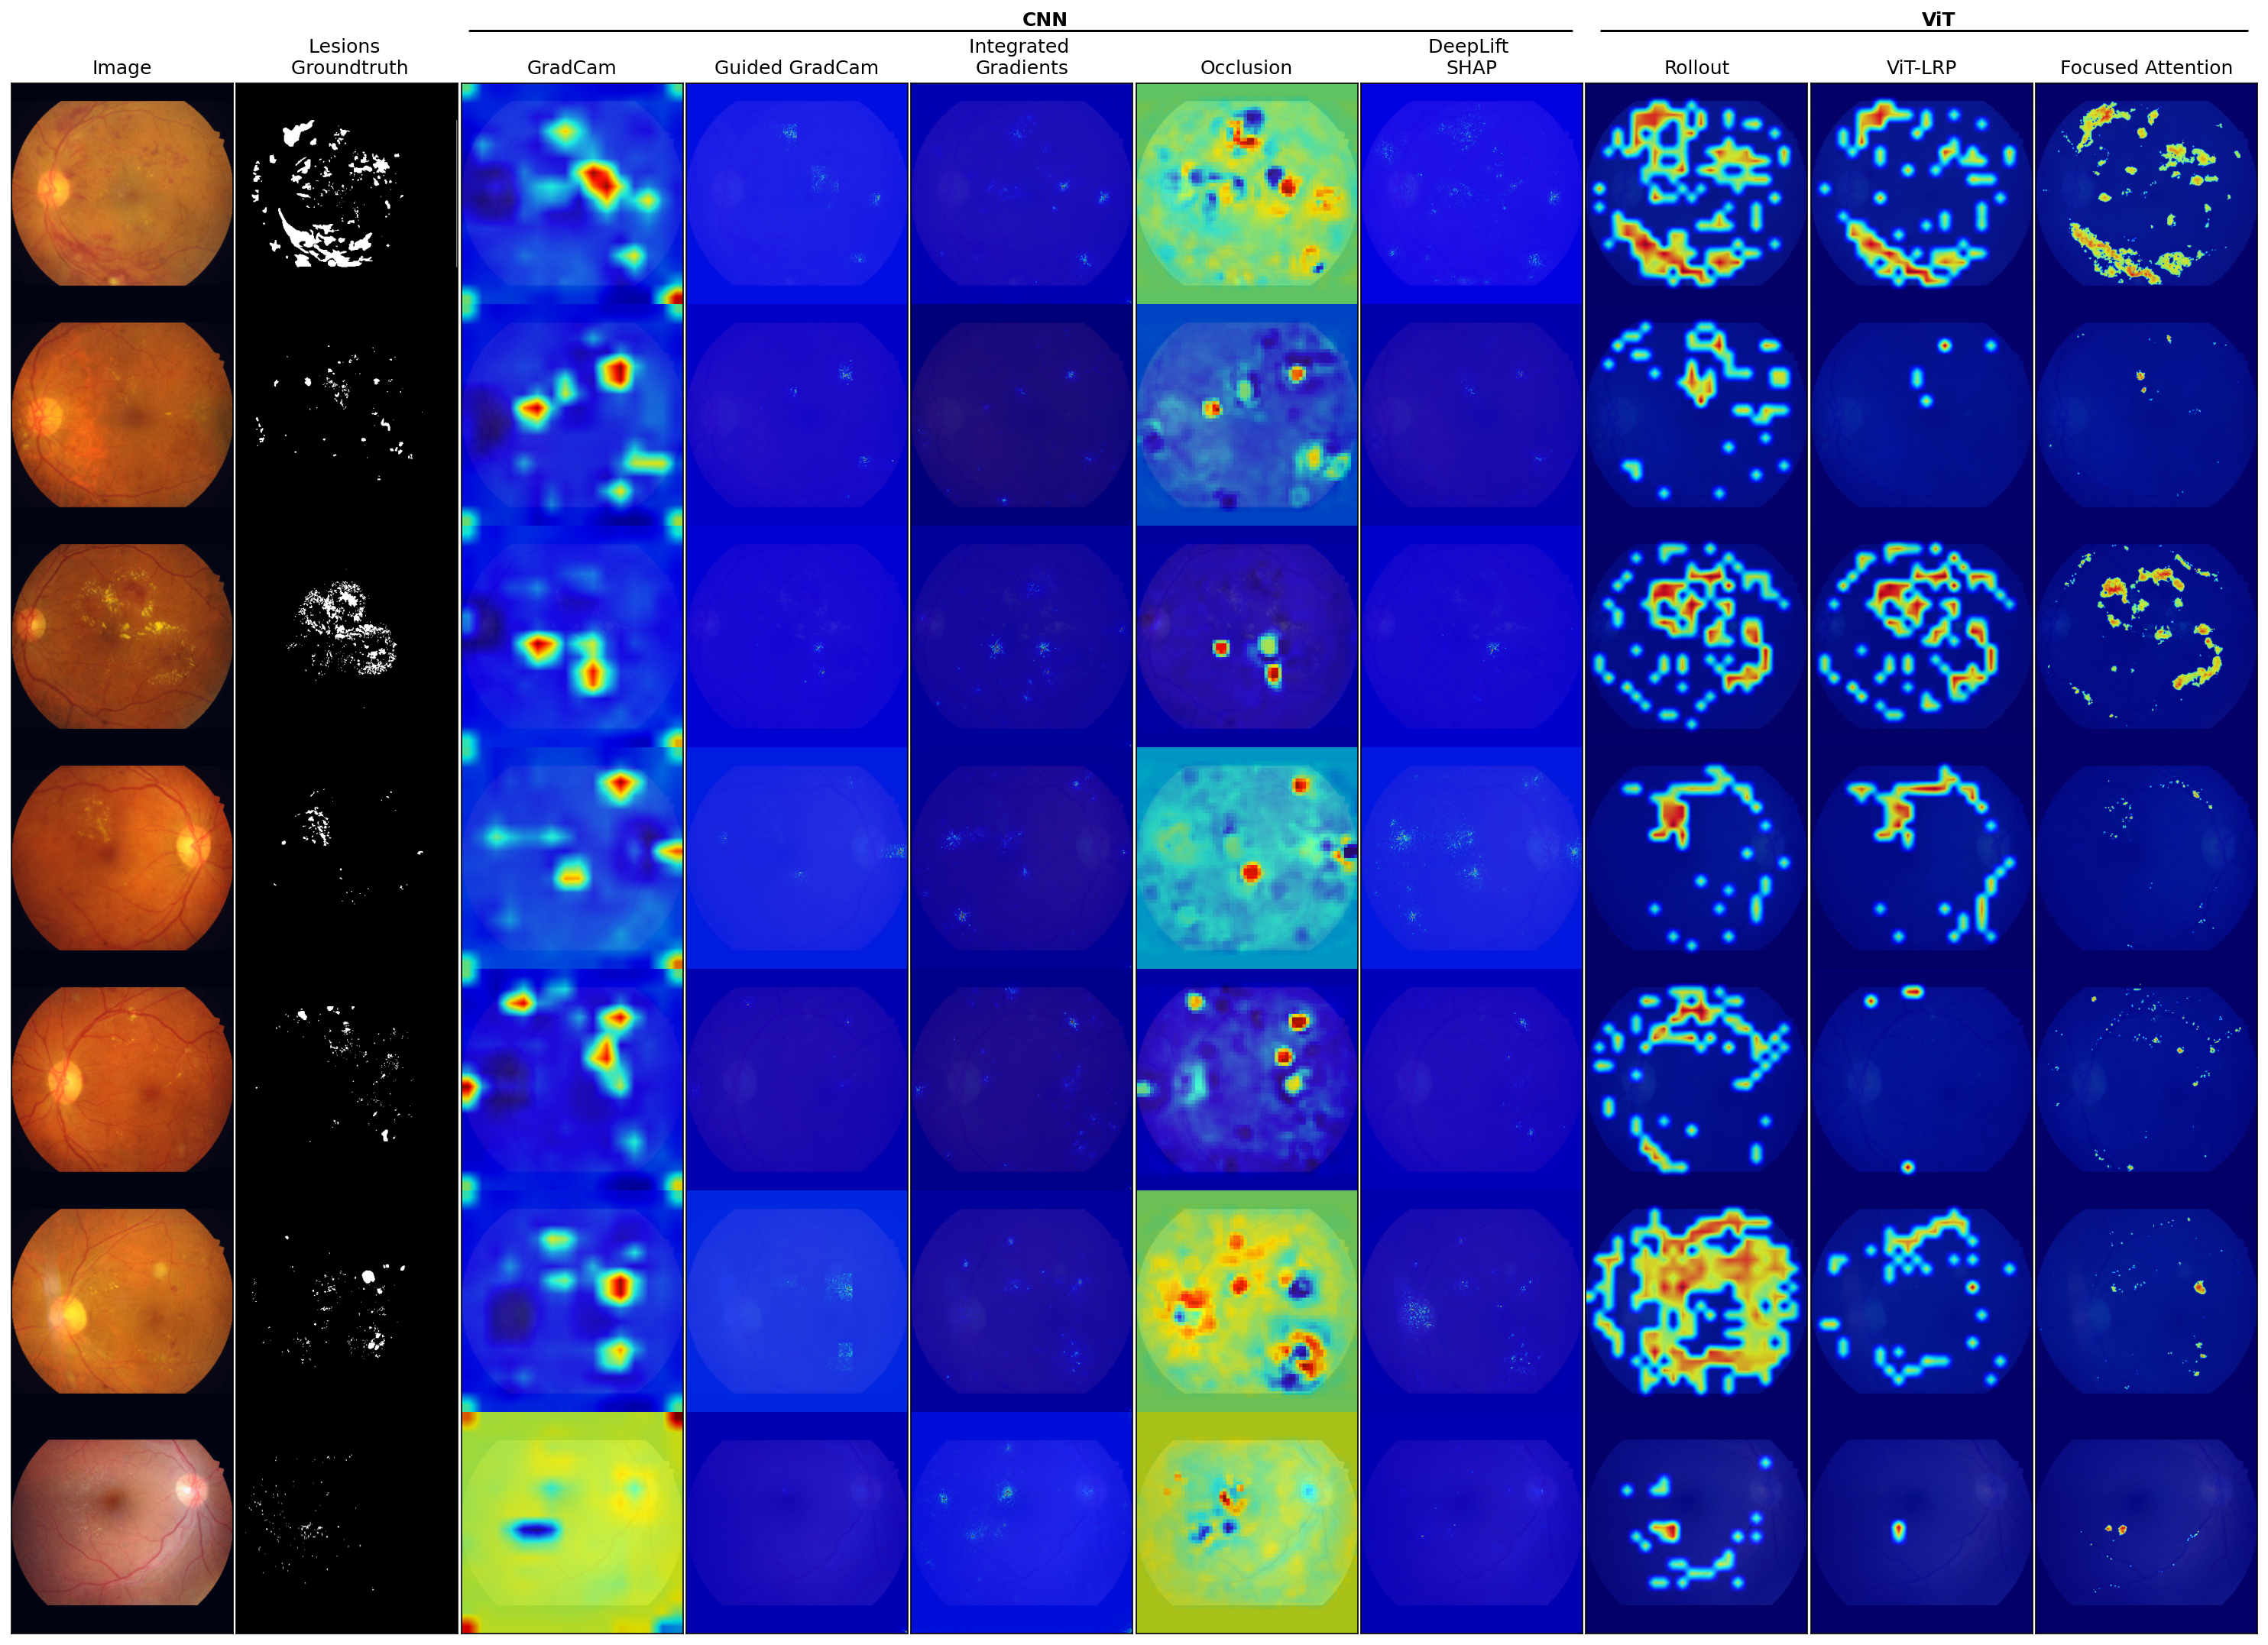
\includegraphics[width=1\linewidth]{gnuplot/focused_attention/interpretability_comparisons/mosaic}
	\caption{Analyse des cartes d'attributions issues de différents algorithmes sur des images de \fundus{} tirées de la base IDRID.}
	\label{fig:mosaic}
\end{figure}



\section{Discussion}
\label{sec:discussionFocusedAttention}
Notre étude souligne les nombreuses forces mais aussi les faiblesses des modèles basés sur le principe du réseau auto-attentif de type Transformer. Nous avons observé un net potentiel pour les \ac{VIT} et variants à égaler voire dépasser les performances de classification d'un modèle de type CNNs. Ce résultat est vérifié sur deux modalités très différentes entre elles, ce qui vient donner de la crédibilité à cette observation et permet statuer sur la capacité d'adaptation de ce type d'architecture. En revanche, en termes d'inférence sur des images d'évaluation non-issues de la même distribution que celles d'entraînement, notre expérience sur la base \ac{HMR} témoigne que les \ac{VIT} ne généralisent pas nécessairement mieux que les CNNs: dans notre cas, la dégradation des performances entre ces deux architectures est très similaire. Ce constat ne s'applique en revanche pas aux T2T-ViT qui parviennent à réduire cet écart de généralisation. En revanche, leurs performances sont globalement moindres, quelle que soit la base de donnée. \\
Un aspect qui semble légèrement distinguer le comportement des CNNs avec celui des \ac{VIT} a trait à l'évolution des performances en fonction du nombre de données d'entraînement. En particulier, on a observé, sur le \fundus{} une plus grande capacité d'amélioration des performances des \ac{VIT} par rapport aux CNNs en augmentant la taille de la base d'apprentissage (+ 2.8\% pour les premiers contre +1.73\% pour les seconds). Ce résultat encourage donc une mise à l'échelle plus grande et donc à la constitution de plus grandes bases de données. Quoiqu'il en soit, en l'état, nos expériences ne permettent pas de conclure sur une supériorité indiscutable d'une approche par rapport à l'autre, du moins en ce qui concerne les métriques d'évaluation communément utilisées.
\\
En revanche, les \ac{VIT}s se démarquent des \ac{CNN}s sur l'interprétabilité de leur prédiction. Ce résultat est largement vérifié sur les deux modalités, quelle que la méthode utilisée pour générer les cartes d'attributions. Pour nous en assurer, nous avons à la fois interrogé des médecins sur leur appréciation des différentes cartes pour aboutir à des conclusions similaires. 
\section{Analyse d'impact et limitations}
Au delà des considérations générales sur les performances de modèles existants (CNNs ou ViT), notre contribution -le pas adaptatif et son extension l'Attention Concentrée- mérite quelques considérations. L'impact à la fois sur les performances (métriques brutes) et sur la qualité des cartes d'attributions est largement démontré, tout particulièrement sur les images de \fundus{}. Certes, les attributions générées sont loin d'égaler la précision des cartes obtenues avec un modèle de segmentation, mais elles s'en approchent plus que jamais. Les résultats qualitatifs (figures \ref{fig:FocusedAttentionExamples} et \ref{fig:mosaic}) nous confortent dans l'idée du potentiel de l'approche, même si par ailleurs les gains quantitatifs (par rapport aux méthodes existantes) paraissent relativement peu élevés en comparaison. Pour autant, à l'origine, la méthode de l'Attention Concentrée souffrait de plusieurs limitations qu'il est important de relever:
\begin{itemize}
	\item Dans sa forme présentée ici, cette technique est relativement lente et coûteuse en ressources computationnelles. La raison est qu'en l'état, elle n'est pas parallélisable, autrement dit, l'algorithme d'Attention Concentrée décrit ici ne peut s'appliquer qu'image par image (et non par \textit{mini-batch})
	\item De plus, l'Attention Concentrée n'est utilisée que pour la génération a posteriori de cartes d'attributions, c'est-à-dire sur un modèle déjà entraîné. Or, l'échantillonnage conditionnel de jetons suivant une distribution probabiliste d'importance devrait, \textit{a priori} bénéficier à l'entraînement également. 
\end{itemize}

Nous insistons sur ce dernier point: l'utilisation de l'Attention Concentrée à l'inférence et pour la génération de cartes d'attributions seulement est une restriction forte du potentiel de la méthode qui ne se justifie que pour des raisons purement techniques (notamment l'absence de parallélisation). En théorie, une architecture devrait bénéficier de cette technique aussi bien pour l'inférence que l'aprentissage: l'introduction d'une forme de stochasticité dans le réseau est une forme de régularisation conduisant bien souvent à une meilleure généralisation; elle peut être comparée en cela à une forme de \textit{Dropout} conditionnel. Par ailleurs, concentrer l'entraînement des ViT sur les jetons d'importance semble être une approche pertinente pour accélérer l'apprentissage: plusieurs travaux s'y sont d'ailleurs depuis intéressés (Liang et al. \cite{liangNotAllPatches2022a}, Yue et al. \cite{yueVisionTransformerProgressive2021}, Xu et al. \cite{evo-vit}). Ces travaux, menés soit simultanément ou après les nôtres, n'utilisent cependant ni le pas adaptatif (permettant une approche multi-résolution de la classification) ni l'échantillonnage conditionnel (comme régularisation stochastique). Nos futurs travaux se concentreront donc sur une adaptation de l'Attention Concentrée pour la rendre fonctionnelle à l'apprentissage. Nous avons d'ors-et-déjà développé une nouvelle version de l'algorithme le rendant parallélisable et optimisant très significativement son fonctionnement. L'entraînement d'un ViT de cette manière entraîne des améliorations substantielles des performances. Cependant, une des principales difficulté est de générer une carte d'échantillonnage conditionnelle durant l'apprentissage; nos futurs travaux se concentreront donc sur cet aspect. 
